\documentclass[a4paper,twocolumn,10pt]{onepgnote}
\usepackage{fontspec} % WICHTIG FÜR LuaLaTeX!
\setmainfont{Latin Modern Roman} % oder eine andere Systemschriftart
\usepackage{dsfont, amsmath}
\usepackage[margin=10pt]{geometry}
\usepackage{yhmath}
\usepackage{tikz}
\usepackage{pifont}
\usepackage{pgfplots}
\pgfplotsset{compat=1.18}
\usepackage{tcolorbox}

\renewtcbox{\notebox}{%
  colback=yellow,      % Hintergrundfarbe
  colframe=yellow,     % Rahmenfarbe
  sharp corners,       % eckige Ecken
  nobeforeafter,       % kein Abstand davor/danach
  box align=base,      % Ausrichtung zur Grundlinie
  size=tight           % kompakte Größe
}

\renewcommand\mynote{\notebox{Hinweis:}\ }  % Ersetzt "Note" durch "Hinweis"
\newcommand{\kariert}[3]{
    \footnotesize #1 \normalsize\newline
    \begin{tikzpicture}
    \draw[step=0.5cm,color=gray] (0,0) grid (#2 cm ,#3 cm);
    \end{tikzpicture}}
\begin{document}
% no header, no footer.
\pagestyle{empty}
\section{Analysis}
\subsection{Grundlagen:}
\begin{itemize}
\item Binomische Formeln\\
\begin{enumerate}
\item $(a+b)^2 = a^2+2\cdot a\cdot b + b^2$\\
\item $(a-b)^2 = a^2 -2\cdot a\cdot b + b^2$\\
\item $(a+b)(a-b) = a^2 - b^2$
\end{enumerate}
\item Potenzengesetze\\
\begin{enumerate}
\item $a^r \cdot b^r = (a\cdot b)^r$ und $\frac{a^r}{b^r} = \left(\frac{a}{b}\right)^r$\\
\item $a^r \cdot a^s = a^{r+s}$ und $ \frac{a^r}{a^s} = a^{r-s}$\\
\item $(a^r)^s = a^{r\cdot s}$\\
\item $a^{\frac{m}{n}} = \sqrt[n]{a^m} = (\sqrt[n]{a})^m$\\
\item $a^{-r} = \frac{1}{a^r}$
\end{enumerate}
\item Logarithmengesetze\\
\begin{enumerate}
\item $\log_a(b\cdot c) = \log_a(b) + \log_a(c)$\\
\item $\log_a(\frac{b}{c}) = \log_a(b) - \log_a(c)$\\
\item $\log_a(b^r) = r\cdot \log_a(b)$\\
\item $\ln(x) = \log_e(x) \longrightarrow \ln(e^x) =x $\\
\item $\operatorname{ld}(x) = \log_2(x)$\\
\item $\operatorname{lg}(x) = \log_{10}(x)$
\end{enumerate}
\end{itemize}
\subsection{Lineare Transformationen:}\\
Wir erhalten aus dem Graphen $G_f$ der Funktion f den Graphen der Funktion g mit:\\
\begin{enumerate}
    \item $g(x) = - f(x)$, indem man $G_f$ an der x--Achse spiegelt\\
\item $g(x) =f(-x)$, indem man $G_f$ an der y--Achse spiegelt\\
\item $g(x) = f(x) +a$ indem man $G_f$ in Richtung der y--Achse um a verschiebt\\
\item $g(x) =f(x-a)$ indem man $G_f$ in Richtung der x--Achse um a verschiebt\\
\item $g(x) =a\cdot f(x)$ und $a>0$, indem man $G_f$ in Richtung der y--Achse mit dem Faktor a streckt bzw. staucht\\
\item $g(x) =f(a\cdot x)$ und  $a>0$, indem man $G_f$ in Richtung der x--Achse mit dem Faktor $\frac{1}{a}$ staucht bzw. streckt.\\

\end{enumerate}

\subsection{Ableitungen:}\\
\begin{enumerate}
\item jede Ableitung ist mit der $h-$Methode nachweisbar $$f'(x) = \lim \limits_{h\longrightarrow 0} \frac{f(x+h) - f(x)}{h}$$
\item $f(x)= c$ mit $c \in\mathds{R} \longrightarrow f'(x) = 0$\hfill\\
\item $f(x)= x  \longrightarrow f'(x) = 1$\\
\item $f(x) = c\cdot x $ mit $c\in\mathds{R}\longrightarrow f'(x) = c$ \\
\item $f(x) = m\cdot x + t  \hspace{0.2cm}\text{mit} \hspace{0.2cm} m,t \in \mathds{R}\longrightarrow f'(x) = m$\\
\item $f(x) = a\cdot g(x)\hspace{0.2cm}\text{mit} \hspace{0.2cm} a \in \mathds{R} \longrightarrow f'(x) = a\cdot g'(x)$ \\
\item $f(x)= g(x) \pm h(x) \longrightarrow f'(x) = g'(x)\pm h'(x)$\\
\item $f(x) = x^n$ mit $n\in \mathds{Q} \longrightarrow f'(x) = n\cdot x^{n-1}$\\
\item $f(x) = g(x) \cdot h(x) \longrightarrow f'(x) = g'(x) \cdot h(x) + g(x) \cdot h'(x)$\\
\item $f(x) = g(h(x)) \longrightarrow f'(x) = g'(h(x)) \cdot h'(x)$\\
\item $f(x) = \dfrac{z(x)}{n(x)} \longrightarrow f'(x) = \dfrac{n(x)\cdot z'(x) - z(x) \cdot n'(x)}{(n(x))^2}$\\ Eselsbrücke\footnote{N-Nenner, Z-Zähler, AZ - Ableitung Zähler, AN - Ableitung Nenner} : $f'(x)=\dfrac{N\cdot AZ-Z\cdot AN}{N^2}$
\end{enumerate}
\subsection{Ableitung spezieller Funktionen:}
\begin{itemize}
\item Trigonometrische Funktionen\\
\begin{enumerate} \item $f(x)= \sin{x} \longrightarrow f'(x) = \cos(x)$\\
\item $f(x)= \cos(x) \longrightarrow f'(x) = -\sin(x)$\\
\item $f(x) = \tan(x)= \dfrac{\sin(x)}{\cos(x)}$ \\$ \longrightarrow f'(x) = \dfrac{\cos(x) \cdot \cos(x) + \sin(x) \cdot \sin(x)}{(\cos(x))^2} = \dfrac{1}{(\cos(x))^2}$
\end{enumerate}
\item e-Funktion\\ \begin{enumerate} \item $f(x) = e^x \longrightarrow f'(x) = e^x$ \\ \item $f(x) = e^{h(x) } \longrightarrow f'(x) = h'(x) \cdot e^{h(x)}$\end{enumerate}
\item ln-Funktion\\ \begin{enumerate} \item $f(x) = \ln(x)$ mit $x\in \mathds{R}^+ \longrightarrow f'(x) = \dfrac{1}{x}$ \end{enumerate}
\item Wurzel\\ \begin{enumerate}\item $f(x) = \sqrt{x} = x^{\frac{1}{2}} \longrightarrow f'(x) = \dfrac{1}{2} \cdot x^{-\frac{1}{2}} = \frac{1}{2\sqrt{x}}$\\ \item $f(x)= \sqrt[n]{x} = x^{\frac{1}{n}} \longrightarrow f'(x) = \frac{1}{n} \cdot x^{\frac{1}{n} -1} = \frac{1}{n\cdot \sqrt[{n-1}]{x}}$\end{enumerate}
\end{itemize}
\subsection{Anwendung der 1. Ableitung}
\begin{itemize}
\item Zusammenhang Steigung $m$ des Graphen $G_f$ einer Funktion $f$ an der Stelle $x_0 \in G_f$ mit der 1. Ableitung:\\
\begin{enumerate}
\item $f'(x_0) = m$\\
\item $\tan{(\alpha)} = m \longrightarrow \alpha = \tan^{-1}{(m)}$
\end{enumerate}
\item Gleichung der Tangente $y_T$ durch den Punkt $P(x_0|f(x_0)) \\y_T = f'(x_0)\cdot(x-x_0) + f(x_0) $
\end{itemize}
\subsection{Grenzwerte spezieller Funktionen:}
\begin{itemize}
\item Ist $p(x)$ ein Polynom, so gilt $\lim \limits_{x\longrightarrow \infty} \frac{p(x)}{e^x} = 0 \longrightarrow e-$Funktion.
\item Ist $p(x)$ ein nicht konstantes Polynom, so gilt \\$\lim \limits_{x\longrightarrow \infty} \frac{\ln(x)}{p(x)} = 0 \longrightarrow ln-$Funktion.
\item Ist $p(x)$ ein Polynom ohne konstanten Summanden , so gilt \\$\lim \limits_{x\longrightarrow 0} (p(x)\cdot \ln(x)) = 0\longrightarrow ln-$Funktion.
\end{itemize}
\subsection{Funktionsklassen:}
\subsubsection{Lineare Funktionen} 
\begin{itemize}
\item Funktionsterm: $f(x) = m\cdot x +t$ mit $m\in \mathds{R}\setminus\{0\}$ und $t\in \mathds{R}$ 
  \begin{enumerate}
  \item $m$ – Steigung der Geraden
  \item $t$ – y-Achsenabschnitt
  \end{enumerate}
  \item Graph einer linearen Funktion ist eine Gerade 
  \item Berechnung der Steigung $ m=\frac{\Delta y}{\Delta x}$
  \item Berechnung des y-Achsenabschnittes t $\longrightarrow$ die Steigung $m$ und die Koordinaten eines Punktes $P(x_0|y_0)$ einsetzen und nach $t$ auflösen
\end{itemize}
\subsubsection{Quadratische Funktionen:}
\begin{itemize}
\item allgemeine Form:$f(x) = a\cdot x^2 + b\cdot x +c$ mit $a\in \mathds{R}\setminus \{0\}$ und $b, c \in \mathds{R}$
\item Graph: 
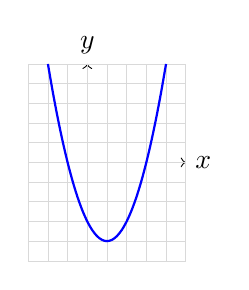
\begin{tikzpicture}[scale=0.25]
  % Achsen
  \draw[->] (-3,0) -- (5,0) node[right] {$x$};
  \draw[->] (0,-5) -- (0,5) node[above] {$y$};
  % Gitter
  \draw[very thin,color=gray!30] (-3,-5) grid (5,5);
  % Parabel: y = x^2 - 2x - 3
  \draw[thick,domain=-2:4,smooth,variable=\x,blue] 
    plot ({\x},{\x*\x - 2*\x - 3});
\end{tikzpicture}
\item Scheitelpunktform: $f(x) = a\cdot(x-x_s)^2 +y_s$ mit $S(x_s|y_s)$ den Koordinaten des Scheitelpunktes
\item Faktorisierte Form: $f(x)= a\cdot (x-x_1)\cdot (x-x_2)$ mit $f(x_1)= 0$ und $f(x_2)= 0$ als Nullstellen der Funktion
\item Nullstellen als Lösung der Gleichung\\ $0 =a\cdot x^2 + b\cdot x +c \longrightarrow x_{1/2} = \dfrac{-b\pm\sqrt{b^2-4\cdot a\cdot c}}{2\cdot a}$
\item Für $a>0$ ist die Parabel nach oben geöffnet $\longrightarrow$ Scheitelpunkt ist Tiefpunkt und es gilt $
\lim\limits_{x \to \pm\infty} f(x) = \infty$
\item Für $a<0$ ist die Parabel nach unten geöffnet $\longrightarrow$ Scheitelpunkt ist Hochpunkt und es gilt $
\lim\limits_{x \to \pm\infty} f(x) = -\infty$\\[0.15cm]
\end{itemize}
\subsubsection{Polynome:}
\begin{itemize}
\item $f(x)= a_n\cdot x^n + a_{n-1} \cdot x^{n-1} + \cdots a_1 \cdot x + a_0 =\sum\limits_{i=0}^{n} a_i x^i$ mit $a_n\in \mathds{R}\setminus \{0\}$ und die restlichen $a_{i} \in \mathds{R}$
\item höchster Exponent legt den Grad des Polynoms fest $\longrightarrow$ hier $n-$ten Grades
\item Beispielgraphen in Abhängigkeit des Grades:\\
\begin{enumerate}\item a gerade: 
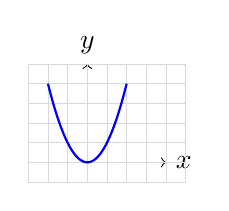
\begin{tikzpicture}[scale=0.25]
  % Achsen
  \draw[->] (-3,0) -- (4,0) node[right] {$x$};
  \draw[->] (0,-1) -- (0,5) node[above] {$y$};
  % Gitter
  \draw[very thin,color=gray!30] (-3,-1) grid (5,5);
  \draw[thick,domain=-2:2,smooth,variable=\x,blue] 
    plot ({\x},{\x*\x});
\end{tikzpicture}
\item a ungerade: 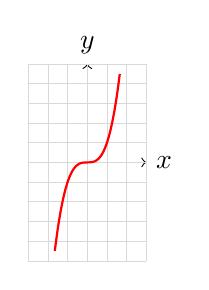
\begin{tikzpicture}[scale=0.25]
  % Achsen
  \draw[->] (-3,0) -- (3,0) node[right] {$x$};
  \draw[->] (0,-5) -- (0,5) node[above] {$y$};
  % Gitter
  \draw[very thin,color=gray!30] (-3,-5) grid (3,5);
     \draw[thick,domain=-1.65:1.65,smooth,variable=\x,red] 
    plot ({\x},{\x*\x*\x});
\end{tikzpicture}\\
\item $n$ gerade und $a_n > 0 \longrightarrow \lim\limits_{x \to \pm\infty} f(x) = \infty$\\
\item $n$ gerade und $a_n <0 \longrightarrow \lim\limits_{x \to \pm\infty} f(x) =- \infty$\\
\item $n$ ungerade und $a_n > 0 \longrightarrow \lim\limits_{x \to -\infty} f(x) = -\infty$ und $ \lim\limits_{x \to \infty} f(x) = \infty$\\
\item $n$ ungerade und $a_n < 0 \longrightarrow \lim\limits_{x \to -\infty} f(x) = \infty$ und $ \lim\limits_{x \to \infty} f(x) = -\infty$
\end{enumerate}
\item ab Grad $n>2$ kennen wir keine Lösungsformel zur Berechnung der Nullstellen\footnote{Für $n=2$ eist das Polynom eine Quadratischen Funktion} $\longrightarrow$ ausklammern bzw. Newton-Verfahren zur Näherung der Nullstellen
\end{itemize}
\subsubsection{Gebrochen-rationale Funktionen}
\begin{itemize}
\item $f(x) = \frac{z(x)}{n(x)}$ und $\mathds{D}_f = \mathds{R}\setminus\{x_i\}$ mit $n(x_i) = 0$
\item Definitionslücken sind die Nullstellen des Nennerpolynoms
\item Nullstellen berechnen sich durch  $0= z(x)$ sind also die Nullstellen des Zählerpolynoms
\item Graph $f(x) = \frac{x^2+1}{x-1} = x+1 +\frac{2}{x-1} $\\
 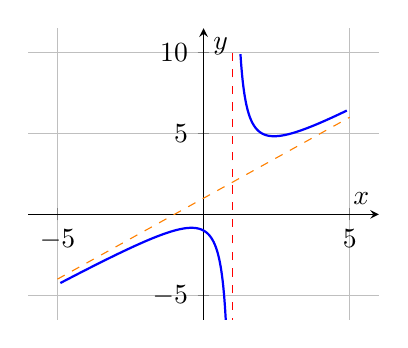
\begin{tikzpicture}
\begin{axis}[
    axis lines=middle,
    xmin=-5, xmax=5,
    ymin=-5, ymax=10,
    samples=400,
    domain=-4.9:4.9,
    restrict y to domain=-10:10,
    enlargelimits=true,
    xlabel={$x$}, ylabel={$y$},
    grid=both,
    scale= 0.65
]

% Die gebrochenrationale Funktion
\addplot[blue, thick, domain=-4.9:0.9, unbounded coords=jump] {(x^2 + 1)/(x - 1)};
\addplot[blue, thick, domain=1.1:4.9, unbounded coords=jump] {(x^2 + 1)/(x - 1)};

% Senkrechte Asymptote x = 1
\addplot[dashed, red] coordinates {(1,-10) (1,10)};
% Schräge Asymptote: y = x + 1
\addplot[dashed, orange, domain=-5:5] {x + 1};
\end{axis}
\end{tikzpicture}\\
\mynote Bei der Monotonie- und Krümmungsuntersuchung muss die Definitionslücke explizit betrachtet werden, an der Definitionslücke kann sich das Monotonie- und Krümmungsverhalten ändern
\item Asymptoten: Die Art der Asymptote einer gebrochen-rationalen Funktion $f(x)=\frac{z(x)}{n(x)}$ mit $\mathds{D} = \mathds{D}_{\text{max}}$ hängt vom Grad der Polynome des Zählers  als auch des Nenners ab\footnote{z-Grad des Zählers; n - Grad des Nenners}.\\
\begin{enumerate}\item z $<$ n: die $x-$Achse ist waagerechte Asymptote $\lim\limits_{x\longrightarrow \infty} f(x) = \lim\limits_{x\longrightarrow -\infty} f(x) = 0$\\
\item  z $=$ n: waagerechte Asymptote die parallel zur x-Achse verläuft $\lim\limits_{x\longrightarrow \infty} f(x) = \lim\limits_{x\longrightarrow -\infty} f(x) = a \in\mathds{R}$\\
\item z $=$ n+1: schräge Asymptote die direkt aus der Summenform ablesbar ist\\
\item z $>$ n +1: Näherungskurve
\end{enumerate}\\

 \end{itemize}
 \subsubsection{$e-$Funktion:}
 \begin{itemize}
 \item $f(x) = e^x$
 \item Graph der Funktion $f(x)= e^x$\\
 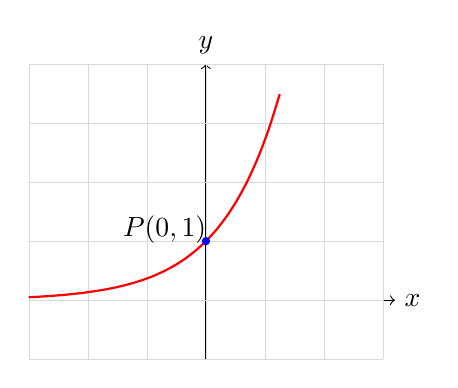
\begin{tikzpicture}[scale=0.75]
  % Achsen
  \draw[->] (-3,0) -- (3.2,0) node[right] {$x$};
  \draw[->] (0,-1) -- (0,4) node[above] {$y$};
  
  % Gitter
  \draw[very thin,color=gray!30] (-3,-1) grid (3,4);
  
  % Funktion e^x
  \draw[thick,domain=-3:1.25,smooth,variable=\x,red] 
    plot ({\x},{exp(\x)});
    % Punkt P(0,1)
  \fill[blue] (0,1) circle (2pt);  % Punkt P(0,1)
  \node at (-0.7,1.2) {$P(0,1)$};  % Beschriftung des Punktes
\end{tikzpicture}
\item Ableitung: $f'(x) = e^x$
\item Grenzwerte:\\
\begin{enumerate}
\item $\lim \limits_{x\longrightarrow -\infty} f(x) = 0$\\
\item $\lim \limits_{x\longrightarrow \infty} f(x) = \infty$
\end{enumerate}
\item $f(x) > 0: $ für alle $x\in \mathds{R}$
\mynote Die $e-$Funktion wächst schneller als jede Potenzfunktion $g(x)= x^n$ mit $n\in\mathds{N}$
\item Bei der Kurvendiskussion wird die $e-$Funktion meistens als Produkt mit einer anderen Funktion betrachtet.\footnote{$f(x) = g(x)\cdot e^{h(x)}  \longrightarrow f'(x) =g'(x)\cdot e^{h(x)} + g(x) \cdot h'(x) \cdot e^{h(x)} $}
 \end{itemize}
 \subsubsection{$ln-$Funktion:}
 \begin{itemize}
 \item $f(x) = \ln(x)$ mit $x\in \mathds{R}^+$
 \item Graph der Funktion $f(x)=\ln(x)$\\
 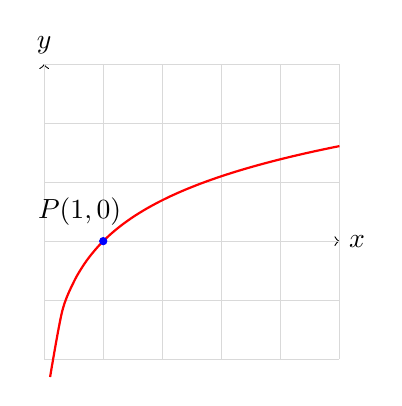
\begin{tikzpicture}[scale=0.75]
  % Achsen
  \draw[->] (0,0) -- (5,0) node[right] {$x$};
  \draw[->] (0,-2) -- (0,3) node[above] {$y$};
  
  % Gitter
  \draw[very thin,color=gray!30] (0,-2) grid (5,3);
  
  % Funktion ln(x)
  \draw[thick,domain=0.1:5,smooth,variable=\x,red] 
    plot ({\x},{ln(\x)});
  
  % Beschriftungen und Punkt (1, 0)
\fill[blue] (1,0) circle (2pt);  % Punkt P(0,1)
  \node at (0.6,0.5) {$P(1,0)$};  % Beschriftung des Punktes
\end{tikzpicture}
\item Ableitung $f'(x) = \frac{1}{x}$
\item Grenzwerte:\\
\begin{enumerate}
\item $\lim \limits_{x\longrightarrow 0^+} f(x) = -\infty$\\
\item $\lim \limits_{x\longrightarrow \infty} f(x) = \infty$
\end{enumerate}
\item \mynote Die $ln-$Funktion wächst langsamer als jede Potenzfunktion $g(x)= x^n$ mit $n\in\mathds{N}$
\item Bei der Kurvendiskussion wird die $ln-$Funktion meistens in Kombination mit einer anderen Funktion betrachtet.\footnote{$f(x) = \ln{(g(x))}  \longrightarrow f'(x) = \dfrac{1}{ g(x)} \cdot g'(x) = \dfrac{g'(x)}{g(x)} $}
 \end{itemize}
 \subsubsection{Wurzelfunktion:}
 \begin{itemize}
 \item $f(x) = a\cdot \sqrt{x-b}+c$ und $x\geq b$ ist eine Halbparabel und ergibt sich durch folgende lineare Transformationen aus der allgemeinen Wurzelfunktion $g(x)= \sqrt{x}$ wie folgt:\\
\begin{enumerate}
    \item Verschiebung um b in x-Richtung\\
    \item Strecken bzw. Stauchen mit dem Faktor a in y-Richtung\\
    \item Verschiebung um c in y-Richtung
\end{enumerate}
\item Graph der Funktion $f(x)= \frac{1}{2} \sqrt{x-2}+2$\\
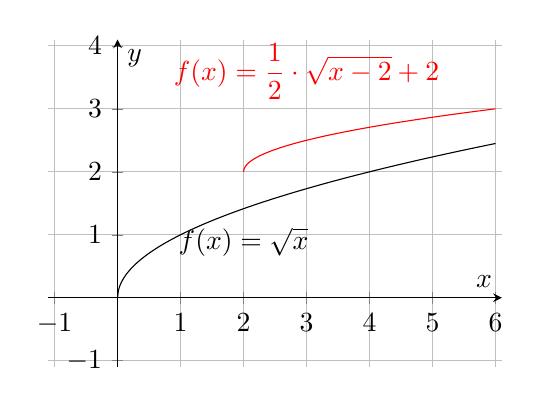
\begin{tikzpicture}
    \begin{axis}[xmin= -1.1, xmax = 6.1, ymin= -1.1, ymax=4.1,
    x=1cm,y=1cm,
        axis lines = middle, 
        ymajorgrids=true,
        xmajorgrids=true,
        xtick={-1,  ..., 6},
        ytick={ -1, ..., 4},
        xlabel = $x$,
        ylabel=$y$, 
        scale= 0.8]      

        \addplot[red, samples = 500, domain= 2:6]{2 + 0.5*(x-2)^(0.5)};
        \draw[red] (3,3)   node [above] {$f(x)=\dfrac{1}{2} \cdot \sqrt{x-2} + 2$};
        \addplot[ samples = 500, domain= 0:6]{(x)^(0.5)};
         \draw (2,0.5)   node [above] {$f(x)= \sqrt{x}$};
    \end{axis}
\end{tikzpicture}
\item Ableitung $f(x)= \sqrt{g(x)} \longrightarrow f'(x) = \frac{g'(x)}{2\cdot \sqrt{g(x)}}$
 \end{itemize}
 \subsubsection{allgemeine Sinusfunktion:} 
 \begin{itemize}
 \item $ f(x)= a\cdot \sin{(b\cdot (x - c))}+d $ mit  $a\in \mathds{R}\setminus\{0\}$ und $b,c,d \in \mathds{R}$
 \begin{enumerate}
\item Der Parameter $a$ ändert die Amplitute, also die maximale Auslenkung der Kurve.\\
\item Der Parameter b streckt bzw. staucht die Kurve in Richtung der x-Achse. Durch den Faktor b wird damit die Periode $p$ verändert $p = \frac{2\cdot \pi}{b}$.\\
        \item Der Parameter c verschiebt die Kurve in Richtung der x-Achse.\\
        \item Der Parameter d verschiebt die Kurve in Richtung der y-Achse.
 \end{enumerate}
 \item Ableitung: $f'(x)=  a\cdot \cos{(b\cdot (x - c))}\cdot b $
 \item Bei der Kurvendiskussion wird die $\sin-$Funktion meistens in Kombination mit einer anderen Funktion betrachtet.\footnote{$f(x) = \sin{(g(x))}  \longrightarrow f'(x) = \cos{(g(x))}\cdot g'(x) $}
 \end{itemize}
 \subsubsection{Betragsfunktionen:}
 \begin{itemize}
     \item Wird eine Funktion $g$ linaren Transformationnen in Form des Betrags unterworfen ergeben sich unterschiedliche Graphen. Diese Graphen haben allerdings gemeinsam, dass die Nicht-Differenzierbarkeit an bestimmten Stellen sich nicht ändert.\\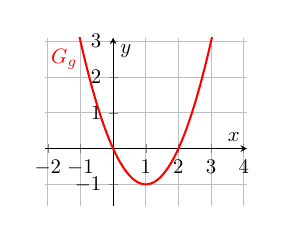
\begin{tikzpicture}[scale=0.75]
    \begin{axis}[xmin= -2.1, xmax = 4.1, ymin= -1.6, ymax= 3.1,
        axis lines = middle, 
        ymajorgrids=true,
        xmajorgrids=true,
        xtick={-2, ..., 4},
        ytick={-2, ..., 3},
        xlabel = $x$,
        ylabel=$y$, scale=0.5]
        \addplot[line width=1pt,mark=none, color=red]  plot[samples=300,smooth]{x^2-2*x};  
        \draw[red] (-1.5,2)   node [above] {$G_{g}$};       
    \end{axis}
\end{tikzpicture}
\item  $g_1(x) = |f(x)|:$ Die Punkte mit negativen Funktionswerten werden an der $x-Achse$ gespiegelt. Die Spiegelung erfolgt damit an den Nullstellen.\\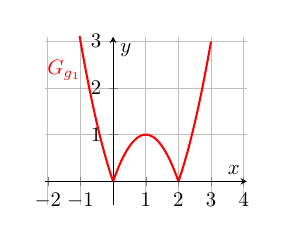
\begin{tikzpicture}[scale=0.75]
    \begin{axis}[xmin= -2.1, xmax = 4.1, ymin= -0.5, ymax= 3.1,
        axis lines = middle, 
        ymajorgrids=true,
        xmajorgrids=true,
        xtick={-2, ..., 4},
        ytick={-2, ..., 3},
        xlabel = $x$,
        ylabel=$y$, scale=0.5]
        \addplot[line width=1pt,mark=none, color=red, restrict x to domain=2:3]  plot[samples=900,smooth]{x^2-2*x}; 
   \addplot[line width=1pt,mark=none, color=red, restrict x to domain=-2:0]  plot[samples=900,smooth]{x^2-2*x};
    \addplot[line width=1pt,mark=none, color=red, restrict x to domain=0.000001:1.99999999999]  plot[samples=900,smooth]{-1*x^2+2*x};
        \draw[red] (-1.5,2)   node [above] {$G_{g_1}$};       
    \end{axis}
\end{tikzpicture}
\item $g_2(x) = f(|x|):$ Der im positive Teil der $x-Achse$ liegende Graaph wird an der $y-Achse$ gespiegelt.\\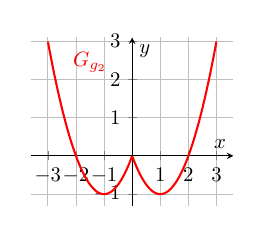
\begin{tikzpicture}[scale=0.75]
    \begin{axis}[xmin= -3.6, xmax = 3.6, ymin= -1.3, ymax= 3.1,
        axis lines = middle, 
        ymajorgrids=true,
        xmajorgrids=true,
        xtick={-3, ..., 4},
        ytick={-2, ..., 3},
        xlabel = $x$,
        ylabel=$y$, scale=0.5]
        \addplot[line width=1pt,mark=none, color=red, restrict x to domain=0:3]  plot[samples=900,smooth]{x^2-2*x}; 
   \addplot[line width=1pt,mark=none, color=red, restrict x to domain=-3:0]  plot[samples=900,smooth]{(-1*x)^2+2*x};
        \draw[red] (-1.5,2)   node [above] {$G_{g_2}$};       
    \end{axis}
\end{tikzpicture}
\item $g_3(x) = |f(|x|)|:$ Wird sowohl der Betrag der $x-Werte$ als auch der Betrag der Funktionswerte gebildet, werden zunächst die Punkte mit positiven $x-$Werten an der $y-$Achse gespiegelt um anschließend die Punkte mit negativen Funktionswerten an der $x-$Achse zu spiegeln.\\ 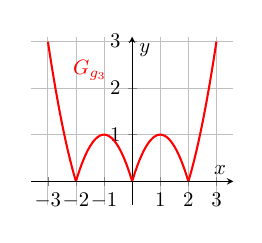
\begin{tikzpicture}[scale=0.75]
    \begin{axis}[xmin= -3.6, xmax = 3.6, ymin= -0.5, ymax= 3.1,
        axis lines = middle, 
        ymajorgrids=true,
        xmajorgrids=true,
        xtick={-3, ..., 4},
        ytick={-2, ..., 3},
        xlabel = $x$,
        ylabel=$y$, scale=0.5]
    \addplot[line width=1pt,mark=none, color=red, restrict x to domain=0:2]  plot[samples=900,smooth]{-1*x^2+2*x};
     \addplot[line width=1pt,mark=none, color=red, restrict x to domain=2:3]  plot[samples=900,smooth]{x^2-2*x}; 
    \addplot[line width=1pt,mark=none, color=red, restrict x to domain=-2:0]  plot[samples=900,smooth]{-1*x^2-2*x};
     \addplot[line width=1pt,mark=none, color=red, restrict x to domain=-3:-2]  plot[samples=900,smooth]{x^2+2*x}; 
        \draw[red] (-1.5,2)   node [above] {$G_{g_3}$};       
    \end{axis}
\end{tikzpicture}
 \item Betragsfunktionen sind an Knickstellen nicht differenzierbar $\longrightarrow$ Nachweis über die $h-$Methode.
 
 \end{itemize}
 \subsection{Kurvendiskussion:}\\
Bei der Kurvendiskussion werden Eigenschaften des Graphen $G_f$ einer Funktion $f$ analytisch untersucht
 \subsubsection{Untersuchung der Ausgangsfunktion:}
 \begin{itemize}
     \item Untersuchung folgender Eigenschaften:\\
     \begin{enumerate}
         \item Definitionsbereich $\longrightarrow$ bei gebrochen-rationalen Funktion z.B. Berechnung der Definitionslücken\\
         \item Schnittpunkte mit den Koordinatenachsen $\longrightarrow$ Nullstellen und Schnittpunkt mit der $y-$Achse\\
         \item Symmetrie zum Ursprung bzw. zur $y-$Achse\\
         \item Verhalten an den Rändern des Definitionsbereichs $\longrightarrow$ Grenzwerte und Verhalten an Definitionslücken\\
         \item Asymptoten
     \end{enumerate}
     \item je nach Funktionsklasse sind die Rechnungen unterschiedlich
 \end{itemize}
 \subsubsection{Monotonie:}
 \begin{itemize}
 \item Ist die Funktion $f$ im Intervall $I$ differenzierbar dann ist $G_f$ für  
 \begin{equation*}
	\left.\begin{aligned}
	f'(x) &>0  \\
	f'(x) &<0
	\end{aligned}
	\right\}
\quad \text{streng monoton}
	\quad\left\{\begin{aligned}
	\text{wachsend}\\
	\text{fallend}
	\end{aligned}
\right.
\end{equation*} 
\item \mynote Für die Existenz einer Extremstellen $x_0 \in G_f$ sind zwei Bedingungen notwendig:\\
\begin{enumerate} \item $f'(x_0)=0$\\
\item $f''(x_0) \neq 0$
\end{enumerate}
\item Die Art der einzelnen Extremstellen läßt sich leicht durch die Vorzeichenwechsel (VZW) der Ableitung an der Stelle $x_0$ mit $f'(x_0)=0$ bestimmen.
 \begin{itemize}
\item Hochpunkt (HoP) $HoP(x_0|f(x_0))$ genau dann, wenn es einen VZW der Ableitung von \textcolor{red}{positiv nach negativ} gibt. \begin{enumerate}\item $f'(x_0) = 0$\\ \item $f''(x_0) < 0$ \end{enumerate}
\item Tiefpunkt (TiP) $TiP(x_0|f(x_0))$ genau dann, wenn es einen VZW der Ableitung von \textcolor{red}{negativ nach positiv} gibt.  \begin{enumerate}\item $f'(x_0) = 0$\\ \item $f''(x_0) > 0$ \end{enumerate}
 \end{itemize}
 \item Untersuchung der Monotonie und der Extremstellen\\
 \begin{enumerate}
     \item Bestimmung der Nullstelle der 1. Ableitung\\
     \item Untersuchung der Monotonie mit Hilfe der Monotonietabelle\\
     \item Entscheidungen zu möglichen Extremstellen
 \end{enumerate}
 \item Monotonietabelle: Eintragung der Intervalle die durch die Nullstellen von $f'(x_1)= 0$ und $f'(x_2)=0$ festgelegt werden.\\
\mynote Beispiel mit zwei Nullstellen:\\\scalebox{0.75}{\begin{tabular}{||c|c|c|c|c|c||}
    \hline
    $x$& $ -\infty <x<x_1 $ & $ x =x_1$ &$ x_1<x<x_2 $ & $x =x_2 $& $ x_2<x<\infty $\\
    \hline \hline
    $f'(x)$ & + & 0 & - & 0 & +\\ 
    \hline
    $G_f$ & smw & $HoP$ & smf & $TiP$& smw\\
    \hline
\end{tabular}}
 \end{itemize}
 \subsubsection{Krümmungsverhalten:}
 \begin{itemize}
     \item Der Punkt, an dem sich die Krümmung des Graphen der Funktion $f$ ändert, heißt Wendepunkt. 
     \item Am Wendepunkt des Graphen liegt ein Extremwert der lokalen Änderungsrate vor. 
     \item Ein Terrassenpunkt ist ein Wendepunkt mit einer waagerechten Tangente.
     \item Zusammenhang der lokalen Änderungsrate und der Krümmung:\\
     \begin{enumerate}
         \item Ist die Funktion $f$ im Intervall $I$ zweimal stetig differenzierbar und ist für alle $x\in I$ der Funktionswert $f''(x)$ \textcolor{red}{positiv}, dann ist der Graph der Funktion $f$ \textcolor{red}{linksgekrümmt}.\\
         \item Ist die Funktion $f$ im Intervall $I$ zweimal stetig differenzierbar und ist für alle $x\in I$ der Funktionswert $f''(x)$ \textcolor{red}{negativ}, dann ist der Graph der Funktion $f$ \textcolor{red}{rechtsgekrümmt}.
     \end{enumerate}
      \item Untersuchung der Krümmung und der Wendestellen\\
 \begin{enumerate}
     \item Bestimmung der Nullstelle der 2. Ableitung\\
     \item Untersuchung der Krümmung mit Hilfe der Krümmungstabelle\\
     \item Entscheidungen zu möglichen Wendestellen
 \end{enumerate}
     \item Ein Wendepunkt liegt nur vor, wenn sich das Krümmungsverhalten ändert.
     \item Krümmungstabelle: Eintragung der Intervalle die durch die Nullstelle von $f''(x_1)= 0$ festgelegt werden.\\
     \mynote Beispiel mit einer Nullstellen:\\\scalebox{0.85}{
     \begin{tabular}{||c|c|c|c||}
    \hline
    $x$& $ -\infty <x<x_1$ & $x = x_1$ & $ x_1<x<\infty$ \\
    \hline \hline
    $f''(x)$ & - & 0 & +\\
    \hline
    $G_f$ & rechtsgekrümmt & Wendepunkt $WP$ & linksgekrümmt\\
    \hline
    \hline
\end{tabular}}
 \end{itemize}
 \subsubsection{Graph:}
 \begin{itemize}
     \item alle berechneten Punkte werden jetzt im Koordinatensystem markiert um dann einen Graphen zu skizzieren
      \end{itemize}
   \subsection{Beispiel} 
   $f(x)= \dfrac{1}{16} x^4 +\dfrac{1}{4} x^3$ mit $\mathds{D}_f =\mathds{D}_{max}$ 
     \begin{itemize}
         \item Bestimmung des maximalen Definitionsbereichs: $\mathds{D}_f = \mathds{R}$ 
         \item Untersuchungen der Symmetrie:
    $$f(-x) = \frac{1}{16} \cdot (-x)^4 + \frac{1}{4} \cdot (-x)^3 = \frac{1}{16} \cdot x^4 - \frac{1}{4} \cdot x^3 \neq \pm f(x)$$ Damit ist der Graph $G_f$ weder punktsymmetrisch zum Ursprung noch achsensymmetrisch zur y-Achse.
    \item Verhalten an den Rändern des Definitionsbereichs
    $$\lim_{x\rightarrow \infty} f(x) = \lim_{x\rightarrow \infty} \dfrac{1}{16}x^4 +\dfrac{1}{4}x^3 = \infty$$
        $$\lim_{x\rightarrow -\infty} f(x) = \lim_{x\rightarrow -\infty} \dfrac{1}{16}x^4 +\dfrac{1}{4}x^3 = \infty$$
    \item Gemeinsame Punkte mit den Koordinatenachsen:\\
    \begin{enumerate}
    \item Schnittpunkt mit der y-Achse $\longrightarrow f(0) = \dfrac{1}{16}0^4 +\dfrac{1}{4}0^3 = 0$ \\
    \item Schnittpunkte mit der x-Achse $\longrightarrow 0 = \dfrac{1}{16} x^3 (x+4) \\\longrightarrow SP_{x_1} = SP_{x_2} = SP_{x_3}(0|0)$ und $SP_{x_4}(-4|0)$
    \end{enumerate}
    \item Monotonie des Graphen\\
    \begin{enumerate}
    \item 1. Ableitung $f'(x)= \dfrac{1}{4} x^3 +\dfrac{3}{4} x^2$\\
    \item Berechnung der Nullstellen der 1. Ableitung\\
    \item  $0 = \dfrac{1}{4} x^3 +\dfrac{3}{4} x^2 \longrightarrow x_1 =x_2 = 0$ und $x_3= -3$\\
\item Monotonietabelle:\\
\scalebox{0.65}{\begin{tabular}{||c|c|c|c|c|c||}
    \hline
    $x$& $ -\infty <x<-3 $ & $ x = -3$ &$ -3<x<0 $ & $x=0 $& $ 0<x<\infty $\\
    \hline \hline
    $f'(x)$ & - & 0 & + & 0 & +\\ 
    \hline
    \hline
    $G_f$ & smf & $TiP(-3|-\frac{27}{16})$ & smw  & $TP(0|0) $& smw\\
    \hline
\end{tabular}}\\
    \end{enumerate}
    \item Krümmungsuntersuchung:\\
    \begin{enumerate}
    \item 2. Ableitung $f''(x) = \dfrac{3}{4} x^2 + \dfrac{3}{2} x$\\
    \item Berechnung der Nullstellen der 2. Ableitung\\
    \item $0 = \dfrac{3}{4} x^2 +\dfrac{3}{2} x \longrightarrow x_1 = 0$ und $x_2= -2$\\
    \item Krümmungstabelle\\
    \scalebox{0.65}{
    \begin{tabular}{||c|c|c|c|c|c||}
    \hline
    $x$ & $ -\infty <x<-2 $ & $ x = -2$ &$ -2<x<0 $ & $x=0 $& $ 0<x<\infty $\\
    \hline \hline
    $f''(x)$ & + & 0 & - & 0 & +\\ 
    \hline
    \hline
    $G_f$ & linksgekr. & $WP(-2|-1)$ & rechtsgekr. & $WP(0|0) $& linksgekr.\\
    \hline
\end{tabular} 
}
    \end{enumerate}
    \item Berechnung der Wendetangente am Punkt $P(-2|-1)$: \\
    \begin{enumerate}
    \item Steigung an der Wendestelle $x_0 = -2$ durch $f'(-2) = 1$\\
    \item einsetzen in $y_T = f'(x_0)\cdot(x-x_0) + f(x_0)\\ \longrightarrow y_T = 1\cdot \left(x-\left(-2\right)\right) +(-1)= x+1$
    \end{enumerate} 
    \item Wertemenge $\mathds{W}= [-\dfrac{27}{16} \hspace{0.1cm}|\hspace{0.1cm} \infty \hspace{0.1cm}[ $
    \item Graph:\\ \scalebox{0.8}{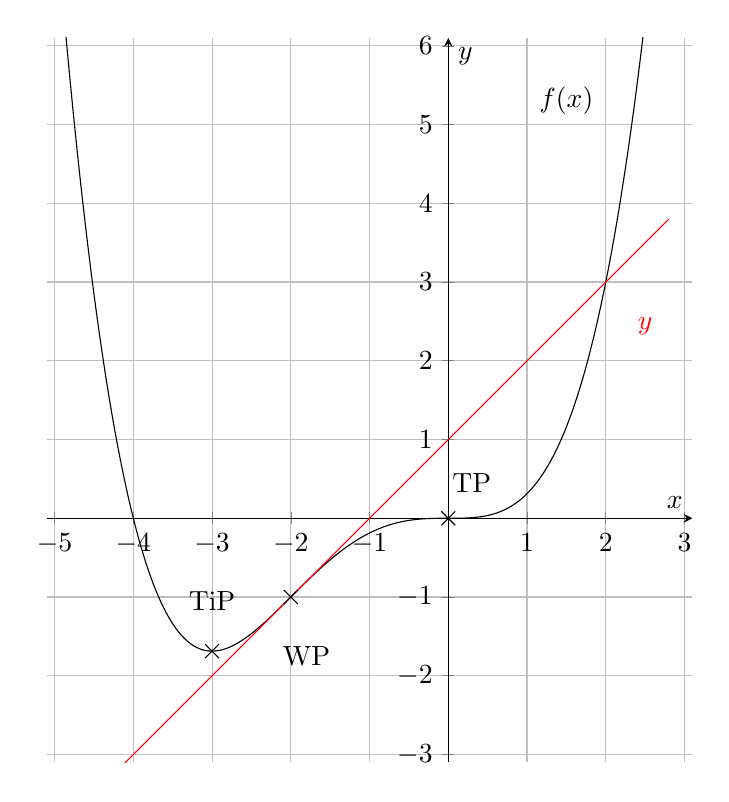
\begin{tikzpicture}
    \begin{axis}[xmin= -5.1, xmax = 3.1, ymin= -3.1, ymax=6.1,
     x=1cm,y=1cm,
        axis lines = middle, 
        ymajorgrids=true,
        xmajorgrids=true,
        xtick={-5, -4, -3,  ..., 3},
        ytick={-3, -2, ..., 6},
        xlabel = $x$,
        ylabel=$y$]
        \addplot[color= black, samples = 300, domain= -5:2.8]{1/16 * x^4 + 1/4*x^3};
        \addplot[color= red, samples = 300, domain= -4.8:2.8]{x +1};
        \draw (-3,-27/16) -- ++(-2.5pt,-2.5pt) -- ++(5pt,5pt) ++(-5pt,0pt) -- ++(5pt,-5pt);
        \draw (-3,-1.3)   node [above] {TiP};
        \draw (0,0) -- ++(-2.5pt,-2.5pt) -- ++(5pt,5pt) ++(-5pt,0pt) -- ++(5pt,-5pt);
         \draw (0.3,0.2)   node [above] {TP};
        \draw (-2,-1) -- ++(-2.5pt,-2.5pt) -- ++(5pt,5pt) ++(-5pt,0pt) -- ++(5pt,-5pt);
         \draw (-1.8,-2)   node [above] {WP};
        \draw (1.5,5)   node [above] {$f(x)$};
        \draw[red] (2.5,2.2)   node [above] {$y$};

    \end{axis}
\end{tikzpicture}}
\end{itemize}
\subsection{Platz für eigene Notizen:}
\kariert{Notizen:}{10}{15}
\end{document}